% ---
% title: An early-warning model
% tags: finance, bayes, total-probability
% ---

\begin{problem}
	\begin{context}
		A borrower \emph{defaults} when she fails to repay her loan as agreed.
		Banks run \emph{early-warning systems}: statistical models that flag
		borrowers who look likely to default, so that the bank can act in time
		(call the client, restructure the loan, stop new lending). No model is
		perfect: it misses some future defaulters and also flags some good
		borrowers.
	\end{context}
	$2\%$ of a bank's borrowers default within a year. An early-warning model
	flags $90\%$ of the borrowers who will default, but also $5\%$ of those who
	will not default.
	(a) What fraction of all borrowers is flagged?
	(b) A borrower is flagged. What is the probability that she defaults?
	(c) A borrower is not flagged. What is the probability that she defaults?
\end{problem}

\begin{slideproblem}
	$2\%$ of a bank's borrowers default within a year. A model flags $90\%$ of
	the future defaulters and $5\%$ of the other borrowers. (a) What fraction
	of borrowers is flagged? Probability of default for (b) a flagged, (c) a
	not flagged borrower?
\end{slideproblem}

\begin{slides}
	\small
	\exstatement
	\begin{columns}[T]
		\begin{column}{.6\textwidth}
			\setlength{\abovedisplayskip}{3pt}
			\setlength{\belowdisplayskip}{3pt}
			\uncover<2->{\sol $D$ = defaults, $A$ = flagged (alarm).
				Data on the tree: $P(D)=0.02$, $P(A\mid D)=0.9$,
				$P(A\mid D^c)=0.05$.}\\[.5mm]
			\uncover<3->{(a) Defaulter or not (exclusive): total probability,
				\[ P(A)=P(A\mid D)P(D)+P(A\mid D^c)P(D^c) \]}
			\uncover<4->{\vspace*{-3mm}
				\[ =0.018+0.049=0.067. \]}
			\uncover<5->{(b) Bayes: turn the condition around,
				\[ P(D\mid A)=\frac{P(A\mid D)P(D)}{P(A)}
					=\frac{0.018}{0.067}=\frac{18}{67}\approx0.269. \]}
		\end{column}
		\begin{column}{.38\textwidth}
			\centering
			\uncover<2->{%
				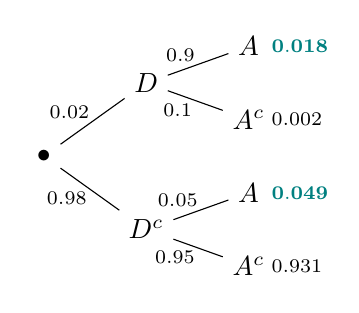
\begin{tikzpicture}[x=1cm,y=.62cm,
						lab/.style={font=\scriptsize,inner sep=1pt}]
					\node (r) at (0,0) {$\bullet$};
					\node (d) at (1.3,1.5) {$D$};
					\node (g) at (1.3,-1.5) {$D^c$};
					\draw (r) -- node[lab,above left] {$0.02$} (d);
					\draw (r) -- node[lab,below left] {$0.98$} (g);
					\node (da) at (2.6,2.25) {$A$};
					\node (dn) at (2.6,.75) {$A^c$};
					\node (ga) at (2.6,-.75) {$A$};
					\node (gn) at (2.6,-2.25) {$A^c$};
					\draw (d) -- node[lab,above left] {$0.9$} (da);
					\draw (d) -- node[lab,below left] {$0.1$} (dn);
					\draw (g) -- node[lab,above left] {$0.05$} (ga);
					\draw (g) -- node[lab,below left] {$0.95$} (gn);
					\node[lab,right,text=teal] at (2.85,2.25) {$\mathbf{0.018}$};
					\node[lab,right] at (2.85,.75) {$0.002$};
					\node[lab,right,text=teal] at (2.85,-.75) {$\mathbf{0.049}$};
					\node[lab,right] at (2.85,-2.25) {$0.931$};
				\end{tikzpicture}}
		\end{column}
	\end{columns}
\end{slides}

\begin{slides}
	\small
	\begin{columns}[T]
		\begin{column}{.45\textwidth}
			\centering
			\textbf{10\,000 borrowers}\\[1mm]
			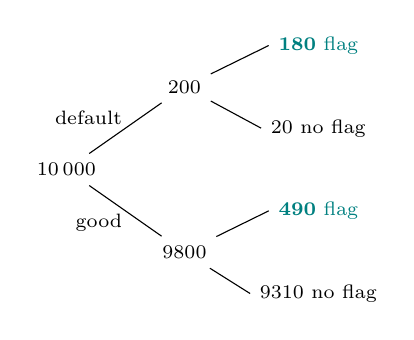
\begin{tikzpicture}[x=1cm,y=.7cm,
					lab/.style={font=\scriptsize,inner sep=1pt}]
				\node (r) at (0,0) {\scriptsize $10\,000$};
				\node (d) at (1.5,1.5) {\scriptsize $200$};
				\node (g) at (1.5,-1.5) {\scriptsize $9800$};
				\draw (r) -- node[lab,above left] {default} (d);
				\draw (r) -- node[lab,below left] {good} (g);
				\node[text=teal] (da) at (3.2,2.25) {\scriptsize $\mathbf{180}$ flag};
				\node (dn) at (3.2,.75) {\scriptsize $20$ no flag};
				\node[text=teal] (ga) at (3.2,-.75) {\scriptsize $\mathbf{490}$ flag};
				\node (gn) at (3.2,-2.25) {\scriptsize $9310$ no flag};
				\draw (d) -- (da.west);
				\draw (d) -- (dn.west);
				\draw (g) -- (ga.west);
				\draw (g) -- (gn.west);
			\end{tikzpicture}
		\end{column}
		\begin{column}{.53\textwidth}
			\uncover<2->{(b) again, with counts: $180+490=670$ borrowers are
				flagged, of whom $180$ default:
				\[ P(D\mid A)=\frac{180}{670}\approx0.269. \]}%
			\uncover<3->{(c) Not flagged: $20+9310=9330$, of whom $20$ default:
				\[ P(D\mid A^c)=\frac{20}{9330}=\frac{2}{933}\approx0.00214. \]}
		\end{column}
	\end{columns}
	\uncover<4->{\smallskip
		\alert{Base rate:} the model is good ($90\%$ of defaulters flagged), yet
		only about $27\%$ of the flags are true. Defaults are rare, so the
		$5\%$ false flags among the many good borrowers ($490$) outnumber the
		true flags ($180$).}
	\uncover<5->{\smallskip
		Still useful: a flag raises the default probability from $2\%$ to
		$27\%$; no flag lowers it to $0.2\%$.}
\end{slides}

\begin{solution}
	\idea Name the events and translate the percentages into (conditional)
	probabilities. The fraction of flagged borrowers comes from the law of total
	probability; the probability of default \emph{given} the flag comes from
	Bayes' formula, which turns the condition around.

	\step{Events and data.} Pick a borrower at random. Let $D$ = ``she
	defaults within a year'' and $A$ = ``the model flags her'' (A for alarm).
	The percentages in the statement are:
	\begin{itemize}[nosep]
		\item $P(D)=0.02$, so $P(D^c)=0.98$;
		\item ``flags $90\%$ of the borrowers who will default'': among the
		      defaulters, $90\%$ are flagged, so $P(A\mid D)=0.9$ and
		      $P(A^c\mid D)=0.1$;
		\item ``flags $5\%$ of those who will not default'': $P(A\mid D^c)=0.05$
		      and $P(A^c\mid D^c)=0.95$.
	\end{itemize}
	Note that $0.9$ is \emph{not} the answer to (b): $P(A\mid D)$ is the
	probability of a flag among defaulters, while (b) asks for the probability
	of default among the flagged borrowers, $P(D\mid A)$.

	\begin{minipage}{.5\linewidth}
		\step{The tree.} First split by default or not, then by flag or not.
		Multiplying along a path gives the probability of that path, e.g.\
		\[ P(DA)=P(D)P(A\mid D)=0.02\cdot0.9=0.018. \]
		The four path probabilities add up to 1.
	\end{minipage}\hfill
	\begin{minipage}{.46\linewidth}
		\centering
		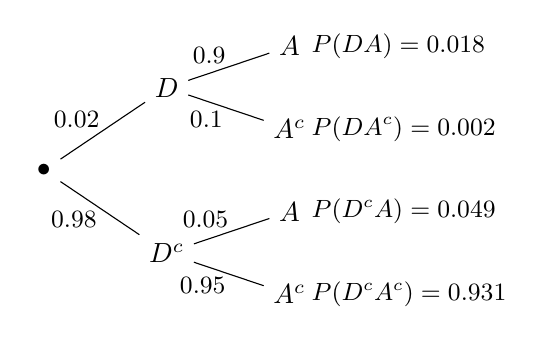
\begin{tikzpicture}[x=1.2cm,y=.7cm,
				lab/.style={font=\small,inner sep=1pt}]
			\node (r) at (0,0) {$\bullet$};
			\node (d) at (1.3,1.5) {$D$};
			\node (g) at (1.3,-1.5) {$D^c$};
			\draw (r) -- node[lab,above left] {$0.02$} (d);
			\draw (r) -- node[lab,below left] {$0.98$} (g);
			\node (da) at (2.6,2.25) {$A$};
			\node (dn) at (2.6,.75) {$A^c$};
			\node (ga) at (2.6,-.75) {$A$};
			\node (gn) at (2.6,-2.25) {$A^c$};
			\draw (d) -- node[lab,above left] {$0.9$} (da);
			\draw (d) -- node[lab,below left] {$0.1$} (dn);
			\draw (g) -- node[lab,above left] {$0.05$} (ga);
			\draw (g) -- node[lab,below left] {$0.95$} (gn);
			\node[lab,right] at (2.8,2.25) {$P(DA)=0.018$};
			\node[lab,right] at (2.8,.75) {$P(DA^c)=0.002$};
			\node[lab,right] at (2.8,-.75) {$P(D^cA)=0.049$};
			\node[lab,right] at (2.8,-2.25) {$P(D^cA^c)=0.931$};
		\end{tikzpicture}
	\end{minipage}

	\step{(a)} A flagged borrower is either a future defaulter ($DA$) or a good
	borrower ($D^cA$). These two events are mutually exclusive, so their
	probabilities add. This is the law of total probability:
	\[ P(A)=P(A\mid D)P(D)+P(A\mid D^c)P(D^c)
		=0.9\cdot0.02+0.05\cdot0.98=0.018+0.049=0.067. \]
	So $6.7\%$ of all borrowers are flagged.

	\step{(b)} We know that the borrower is flagged, so the condition is $A$.
	By the definition of conditional probability,
	$P(D\mid A)=P(DA)/P(A)$. The numerator is the path ``defaults and is
	flagged'' of the tree, the denominator is the result of (a). This is
	Bayes' formula:
	\[ P(D\mid A)=\frac{P(A\mid D)P(D)}{P(A\mid D)P(D)+P(A\mid D^c)P(D^c)}
		=\frac{0.018}{0.067}=\frac{18}{67}\approx0.269. \]

	\step{(c)} Now the condition is $A^c$, ``not flagged''. By the complement
	rule, $P(A^c)=1-0.067=0.933$. Among the two paths that end in $A^c$, the
	borrower defaults on the path $DA^c$, with probability
	$P(D)P(A^c\mid D)=0.02\cdot0.1=0.002$. So
	\[ P(D\mid A^c)=\frac{P(A^c\mid D)P(D)}{P(A^c)}=\frac{0.002}{0.933}
		=\frac{2}{933}\approx0.00214. \]

	\step{Check with frequencies.} Imagine $10\,000$ borrowers. About $2\%$ of
	them, $200$, will default; $9800$ will not. Of the $200$ defaulters the
	model flags $90\%$, that is $180$ (and misses $20$). Of the $9800$ good
	borrowers it flags $5\%$, that is $490$ (and does not flag $9310$).
	\begin{itemize}[nosep]
		\item Flagged: $180+490=670$ borrowers, $6.7\%$ of all (part (a)).
		\item Of the $670$ flagged, $180$ default: $180/670\approx0.269$
		      (part (b)).
		\item Not flagged: $20+9310=9330$, of whom $20$ default:
		      $20/9330\approx0.00214$ (part (c)).
	\end{itemize}
	\begin{answer}
		(a) $0.067$ \quad (b) $\frac{18}{67}\approx0.269$ \quad
		(c) $\frac{2}{933}\approx0.00214$
	\end{answer}
	\begin{remark}
		\textbf{The base-rate effect.} The model catches $90\%$ of the
		defaulters and raises a false alarm for only $5\%$ of the good
		borrowers, yet only about $27\%$ of the flagged borrowers actually
		default. The reason is the low \emph{base rate}: defaults are rare
		($2\%$), so the $5\%$ false alarms come from a very large group ($9800$
		borrowers) and outnumber the true alarms ($490$ against $180$). The model
		is still useful: a flag raises the probability of default from $2\%$ to
		about $27\%$, more than thirteen times, and no flag lowers it to about
		$0.2\%$. Exercise~\exref{medical-test} has the same structure, and
		Exercise~\exref{early-warning-odds} redoes (b) with odds and adds a
		second model.
	\end{remark}
	\begin{remark}
		\textbf{Common mistake:} answering (b) with $0.9$. That is
		$P(A\mid D)$, the probability of a flag \emph{given} default. The
		question asks for $P(D\mid A)$, the probability of default given a
		flag; turning the condition around is exactly what Bayes' formula does.
	\end{remark}
\end{solution}
